\documentclass{article}
\usepackage[a4paper, hmargin=1.5cm, vmargin={2cm,2cm}]{geometry}
\usepackage[utf8]{inputenc}
\usepackage[T1]{fontenc}
\usepackage{amsmath,amssymb}
\usepackage[fontsize=14pt]{scrextend}
\usepackage[brazil]{babel}
\usepackage{graphicx}
\graphicspath{{docs/imgs/experimentos/}{imgs/experimentos/}{../imgs/experimentos/}}
\usepackage{booktabs}
\usepackage{tabularx}
\usepackage{enumitem}
\usepackage{placeins}
\usepackage{amsthm}
\newtheorem{theorem}{Teorema}
\theoremstyle{remark}
\newtheorem*{obs}{Observação}
\newenvironment{observacao}{\begin{obs}\small}{\end{obs}}
\usepackage[hidelinks]{hyperref}

\begin{document}

\pagestyle{empty}

\newpage
\section{Introdução}

O cancelamento de serviços por clientes, conhecido como \textit{churn}, representa um desafio para empresas de telecomunicações, uma vez que pode comprometer receitas e dificultar o planejamento de estratégias de retenção. Nesse contexto, técnicas de aprendizado de máquina (\textit{Machine Learning}) têm sido empregadas na construção de modelos preditivos, permitindo identificar padrões associados ao comportamento dos consumidores e estimar a probabilidade de cancelamento a partir de suas características.\\

Entre as abordagens utilizadas para essa finalidade, destaca-se a regressão logística binária, cujo ajuste aos dados pode ser formulado como um problema de otimização não linear. A determinação dos parâmetros do modelo envolve, portanto, a minimização de uma função objetivo, cuja solução pode ser obtida por diferentes métodos numéricos.\\

Diante disso, o objetivo deste trabalho é investigar a aplicação de métodos de otimização não linear irrestrita na estimação dos parâmetros de um modelo de regressão logística binária para a previsão de cancelamento de clientes, utilizando uma base de dados pública do setor de telecomunicações. Para alcançar esse objetivo, estabelecem-se os seguintes objetivos específicos:

\begin{itemize}
    \item Formular matematicamente o problema de otimização e estudar suas principais propriedades teóricas;
    \item Implementar e comparar os métodos de Cauchy e de Newton Puro na resolução do problema;
    \item Avaliar os resultados numéricos e o desempenho preditivo dos modelos obtidos, utilizando uma implementação de referência \texttt{scikit-learn} para validação 
\end{itemize}

\section{O problema}

Nesta seção, formulamos o problema de estimação dos parâmetros de um modelo de regressão logística binária e apresentamos os resultados teóricos que fundamentam os métodos numéricos empregados em sua resolução. A formulação utiliza como referência os trabalhos de [1--5].

\subsection{Contextualização e Fundamentação Teórica}

A rotatividade de clientes, do inglês churn, denomina, neste trabalho, o cancelamento de serviços por clientes e constitui um fenômeno de interesse para empresas de telecomunicações. A identificação de padrões associados à interrupção dos contratos permite desenvolver modelos estatísticos e de aprendizado de máquina capazes de estimar a probabilidade de cancelamento a partir de informações dos consumidores. A construção de tais modelos exige a definição de um conjunto de variaveis explicativas, cuja escolha pode influenciar tanto o desempenho preditivo quanto a complexidade da solução obtida. \\

Para o desenvolvimento deste trabalho, utilizamos uma base de dados pública e fictícia [1], contendo informações de supostos clientes de uma empresa de telecomunicações. Cada observação corresponde a um cliente, sendo disponibilizadas características demográficas, informações sobre serviços contratados, duração do vínculo com a empresa e dados financeiros. A variável de interesse, \textit{churn}, indica se o cliente interrompeu ou não seus serviços, constituindo a resposta que se deseja prever. \\

Nesse contexto, consideramos o problema de treinar um modelo de regressão logística capaz de estimar a probabilidade de cancelamento a partir da seleção dos atributos disponíveis, evitando o uso de variáveis que carregam informação direta sobre o desfecho, situação conhecida como vazamento de dados (\textit{data leakage}). A partir dos atributos selecionados, buscamos estimar os parâmetros do modelo por meio da minimização de uma função objetivo, formulando, assim, um problema de otimização não linear irrestrita, cuja resolução será investigada por meio dos métodos de Cauchy e de Newton [2]. \\

Além de estudar as propriedades matemáticas da função objetivo, buscamos comparar o comportamento numérico dos métodos na estimação dos parâmetros e avaliar os resultados obtidos em relação a uma implementação de referência [5].

\subsection{Modelagem matemática}\label{subsec:modelagem}

Para a formulação matemática do problema, consideramos um conjunto de $m$ observações, cada uma correspondente a um cliente da empresa de telecomunicações. A cada cliente estão associados um conjunto de atributos explicativos -- parâmetros -- e uma variável resposta binária $y_i \in \{0,1\}$, com $y_i = 1$ indicando o cancelamento do serviço. A relação entre essas variáveis é representada por um modelo de regressão logística binária [3,4].\\

A base [1] possui \textit{N} = 7.043 clientes, dos quais 80\% ($m = 5.634$) formam o conjunto de treino, utilizado na definição da função objetivo e de suas derivadas. Os 1.409 clientes restantes são reservados para a avaliação final. Foram selecionadas nove variáveis explicativas, sendo quatro numéricas, duas binárias e três categóricas, excluindo explicitamente cinco atributos que carregam informação direta sobre o desfecho (\texttt{Churn Score}, \texttt{Churn Category}, \texttt{Churn Reason}, \texttt{Customer Status} e \texttt{Satisfaction Score}), além de identificadores e atributos geográficos. Após codificar as variáveis categóricas em variáveis indicadoras, via \textit{One-Hot Encoding}, com descarte da categoria de referência, padronizar as variáveis numéricas e acrescentar o intercepto, cada cliente é representado por $x_i \in \mathbb{R}^n$, com $n = 14$ ($1$ intercepto, $4$ atributos numéricos e $9$ colunas binárias/indicadoras). O detalhamento completo do pré-processamento é apresentado na Seção~\ref{sec:experimentos}.\\

Denotamos por $X \in \mathbb{R}^{m \times n}$ a matriz cujas linhas são $x_i^{\top}$ ($i = 1, \dots, m$) e por $w = (w_0, w_1, \dots, w_{13})^{\top} \in \mathbb{R}^{14}$ o vetor de pesos, sendo $w_0$ o termo de intercepto. A Tabela~\ref{tab:estrutura_pesos} apresenta a correspondência exata entre cada componente de $w$ e as colunas da matriz $X$.

\begin{table}[ht]
\centering
\caption{Estrutura do vetor de pesos $w \in \mathbb{R}^{14}$ e correspondência com as colunas da matriz $X$.} 
\label{tab:estrutura_pesos}
\renewcommand{\arraystretch}{1.15}
\begin{tabularx}{\textwidth}{@{} l X l @{}}
\toprule
\textbf{Índice do Peso} & \textbf{Atributo Correspondente em $X$} & \textbf{Tipo / Natureza} \\
\midrule
$w_0$ & \texttt{Intercepto} (coluna unitária) & Constante \\
$w_1$ & \texttt{Age} (Idade do cliente, 19 a 80 anos) & Numérica (Z-score) \\
$w_2$ & \texttt{Tenure in Months} (Tempo de vínculo, 1 a 72 meses) & Numérica (Z-score) \\
$w_3$ & \texttt{Monthly Charge} (Valor da mensalidade) & Numérica (Z-score) \\
$w_4$ & \texttt{Number of Referrals} (Quantidade de indicações) & Numérica (Z-score) \\
$w_5$ & \texttt{Paperless Billing} (Fatura digital) & Binária ($\{0,1\}$) \\
$w_6$ & \texttt{Married} (Estado civil) & Binária ($\{0,1\}$) \\
$w_7, w_8$ & \texttt{Contract\_One Year}, \texttt{Contract\_Two Year} & Binárias (One-Hot) \\
$w_9, w_{10}, w_{11}$ & \texttt{Internet Type\_DSL}, \texttt{Fiber Optic}, \texttt{None} & Binárias (One-Hot) \\
$w_{12}, w_{13}$ & \texttt{Payment Method\_Credit Card}, \texttt{Mailed Check} & Binárias (One-Hot) \\
\bottomrule
\end{tabularx}
\end{table}

\begin{observacao}
A padronização das quatro variáveis numéricas foi feita por meio da transformação Z-score:
\[
z_{ij} = \frac{x_{ij} - \bar{x}_j}{s_j},
\]
em que $x_{ij}$ é o valor a ser padronizado, enquanto $\bar{x}_j$ e $s_j$ denotam, respectivamente, a média e o desvio padrão amostrais, calculados exclusivamente sobre o conjunto de treino e aplicados sem recálculo ao conjunto de teste, para evitar vazamento de dados. Essa transformação centraliza os dados em média zero e variância unitária, melhorando o número de condição da matriz Hessiana e permitindo comparar variáveis originalmente medidas em escalas distintas.\\
\end{observacao}

Na regressão logística binária, modela-se o logaritmo da razão de chances de ocorrência do evento de cancelamento como uma combinação linear dos atributos [3, 4]:\\
\[
\ln \left( \frac{P(y_i = 1 | x_i;w)}{1-P(y_i = 1|x_i;w)}\right) = x_i^{\top}w.
\]\\
Denotando a probabilidade estimada de cancelamento por $\hat p_i(w) = P(y_i = 1 | x_i;w)$ e isolando-a na equação anterior, obtém-se a relação dada pela função sigmoide:
\[
\hat p_i(w) = \sigma(x_i^\top w), \qquad \sigma(z) = \frac{1}{1 + e^{-z}}.
\]
Os pesos são estimados por máxima verossimilhança, isto é, minimizando o oposto da log-verossimilhança média, a chamada entropia cruzada:
\[
f(w) = -\frac{1}{m} \sum_{i=1}^{m} \Big[ y_i \ln \hat p_i(w) + (1 - y_i) \ln \big(1 - \hat p_i(w)\big) \Big] = \frac{1}{m} \sum_{i=1}^{m} \Big[ \ln\big(1 + e^{x_i^\top w}\big) - y_i\, x_i^\top w \Big].
\]
Assim, o problema de otimização irrestrito do trabalho é
\begin{equation}
\min_{w \in \mathbb{R}^{14}} f(w) = \frac{1}{m}\sum_{i=1}^{m}\Big[\ln\!\big(1 + e^{x_i^{\top} w}\big) - y_i x_i^{\top} w\Big],
\label{eq:problema}
\end{equation}

em que $w \in \mathbb{R}^{14}$ é o vetor de variáveis de decisão e $f(w)$ mede a discrepância média entre as probabilidades preditas e os desfechos observados no conjunto de treino. \\

\begin{observacao}
A formulação~\eqref{eq:problema} minimiza a entropia cruzada pura, sem termo de penalização ou regularização adicional. A simplicidade e a interpretabilidade do modelo são obtidas previamente pela seleção criteriosa das nove variáveis explicativas no pré-processamento, o que também permite validar diretamente a solução numérica frente à regressão logística não regularizada da biblioteca \texttt{scikit-learn}.
\end{observacao}


\subsection{Métodos de Resolução}\label{subsec:metodos}

Os métodos de Cauchy e de Newton [2] utilizam, respectivamente, o gradiente e a Hessiana da função objetivo. Sejam $\hat p(w) \in \mathbb{R}^m$ o vetor de entradas $\hat p_i(w) = \sigma(x_i^\top w)$, $y \in \{0,1\}^m$ o vetor das respostas e $D(w) = \operatorname{diag}\big(\hat p_i(w)\,(1 - \hat p_i(w))\big)$, cujas entradas pertencem a $(0, 1/4]$. Como $\sigma' = \sigma(1 - \sigma)$, obtemos
\begin{align}
\nabla f(w) &= \frac{1}{m} X^\top \big( \hat p(w) - y \big), \label{eq:grad} \\
\nabla^2 f(w) &= \frac{1}{m} X^\top D(w)\, X. \label{eq:hess}
\end{align}
Portanto, a Hessiana é semidefinida positiva em todo ponto, e sua positividade estrita depende do posto de $X$. As garantias teóricas a seguir utilizam duas hipóteses sobre os dados de treino:
\begin{itemize}
\item[(H1)] A Matriz $\mathit{X}$ possui posto completo de colunas, ou seja, $\operatorname{posto}(X) = n$;
\item[(H2)] Não existe $v \neq 0$ tal que $(2y_i - 1)\, x_i^\top v \geq 0$ para todo $i$, isto é, não há separação linear completa, nem quase completa, entre as classes [3].
\end{itemize}
Ambas são verificadas numericamente sobre os dados de treino (posto e número de condição de $X$; convergência dos métodos com pesos limitados).

\begin{theorem}
\label{teo:existencia}
Suponha que as hipóteses H1 e H2 sejam satisfeitas. Então:
\begin{enumerate}[label=(\roman*)]
    \item $f \in C^{\infty}(\mathbb{R}^n)$ e a Hessiana $\nabla^2 f(w)$ é simétrica e definida positiva ($\nabla^2 f(w) \succ 0$) para todo $w \in \mathbb{R}^n$, de modo que $f$ é estritamente convexa;
    \item $f$ é coerciva ($\lim_{\|w\|_2 \to +\infty} f(w) = +\infty$) e possui um único minimizador global $w^* \in \mathbb{R}^n$, caracterizado pela condição $\nabla f(w^*) = 0$;
    \item o gradiente $\nabla f$ é globalmente Lipschitz contínuo em $\mathbb{R}^n$, com constante
    \[
    L = \frac{\lambda_{\max}(X^{\top}X)}{4m},
    \]
    em que $\lambda_{\max}(X^{\top}X)$ denota o maior autovalor da matriz $X^{\top}X$. \\
\end{enumerate}
\end{theorem} 

\begin{theorem}\label{teo:nivel}
Sob as mesmas hipóteses do Teorema \ref{teo:existencia}, sejam $w^0 \in \mathbb{R}^n$ e $S = \{ w \in \mathbb{R}^n : f(w) \leq f(w^0) \}$. Então $S$ é compacto e convexo, e existe $\mu > 0$ tal que
\[
\mu I \preceq \nabla^2 f(w) \preceq L I \quad \text{para todo } w \in S.
\]
\end{theorem} 

As demonstrações utilizam resultados clássicos de [2] e [3]: a convexidade e a cota de $L$ seguem da estrutura de \eqref{eq:hess} e de $\hat p_i(1 - \hat p_i) \leq 1/4$; a positividade estrita, de $v^\top \nabla^2 f(w)\, v = \frac{1}{m} \sum_i d_{ii} (x_i^\top v)^2$ e de (H1); e a existência, da coercividade de $f$ garantida por (H2) e do Teorema de Weierstrass.

\subsubsection{Método de Cauchy com Busca Linear Exata}

A partir de $w^0$, o método de Cauchy toma como direção de busca o oposto do gradiente e avança até o minimizador de $f$ ao longo dela:
\[
d^k = -\nabla f(w^k), \qquad w^{k+1} = w^k + t_k d^k, \qquad t_k = \arg\min_{t \geq 0} \, \varphi_k(t), \quad \varphi_k(t) = f(w^k + t d^k).
\]
Enquanto $\nabla f(w^k) \neq 0$, $d^k$ é direção de descida, pois $\varphi_k'(0) = -\|\nabla f(w^k)\|^2 < 0$. Pelo Teorema \ref{teo:existencia}, $\varphi_k$ é estritamente convexa e $t_k$ é único. Como não há fórmula fechada para $t_k$, ele é calculado numericamente pelo método da seção áurea [2]: após enquadrar o minimizador em um intervalo, este é reduzido sucessivamente pelos fatores $\theta_1 \approx 0{,}382$ e $\theta_2 \approx 0{,}618$ até a tolerância desejada.\\

Além disso, sob as condições dos Teoremas \ref{teo:existencia} e \ref{teo:nivel}, o resultado clássico de [2] garante a convergência $w^k \to w^*$ para qualquer $w^0$, com
\[
f(w^{k+1}) - f(w^*) \leq \Big( 1 - \frac{\mu}{L} \Big) \big( f(w^k) - f(w^*) \big),
\]
isto é, convergência linear, com razão que depende do condicionamento $L/\mu$. Quando as curvas de nível são alongadas, o método apresenta o comportamento em zigue-zague e exige muitas iterações, o que torna relevante a padronização dos atributos.

\subsubsection{Método de Newton Puro}\label{subsubsec:newton}

O método de Newton minimiza, a cada iteração, o modelo quadrático de $f$ em torno de $w^k$. A direção $d^k$ é a solução do sistema linear
\[
\nabla^2 f(w^k)\, d^k = -\nabla f(w^k), \qquad w^{k+1} = w^k + d^k,
\]
com passo unitário. Sob a hipótese H1, a Hessiana é simétrica e definida positiva em todo ponto, de modo que o sistema tem solução única e $d^k$ é sempre direção de descida:
\[
\nabla f(w^k)^\top d^k = -\nabla f(w^k)^\top \big[ \nabla^2 f(w^k) \big]^{-1} \nabla f(w^k) < 0.
\]
Como $f \in C^\infty$ e $\nabla^2 f(w^*)$ é definida positiva, o método converge quadraticamente quando $w^0$ está suficientemente próximo de $w^*$ [2]. Em contrapartida, o passo unitário não garante decréscimo de $f$ longe da solução, e a versão pura não tem convergência global assegurada. Isso se conecta à saturação da sigmoide: quando $|x_i^\top w|$ é grande, $\hat p_i(1 - \hat p_i)$ aproxima-se de zero, a Hessiana torna-se numericamente quase singular e o passo de Newton pode ser muito grande. \\

Os critérios de parada, os pontos iniciais $w^0$, a comparação numérica entre os métodos e a validação do ponto ótimo frente a uma implementação de referência são apresentados na Seção~\ref{sec:experimentos}.

\section{Experimentos Numéricos}\label{sec:experimentos}

Nesta seção, são apresentados os experimentos numéricos realizados para avaliar o comportamento dos métodos de Cauchy com busca linear via Seção Áurea e de Newton Puro na estimação dos parâmetros da regressão logística binária, tomando a biblioteca \texttt{scikit-learn} como referência numérica. A análise considera a convergência dos algoritmos, o valor da função objetivo, a norma do gradiente, o número de iterações e o tempo de execução, examinando também o efeito da tolerância de convergência, a limitação do número de iterações e a influência do ponto inicial.

Os testes numéricos foram implementados em \texttt{Python 3.13} (utilizando as bibliotecas \texttt{NumPy}, \texttt{Pandas}, \texttt{scikit-learn} e \texttt{Matplotlib}) e executados em um computador com sistema operacional Windows 10 Home (64 bits), processador Intel Core i7-7700K @ 4,20~GHz, 16,0~GB de memória RAM (2400~MHz) e placa de vídeo NVIDIA GeForce GTX 1070 (8~GB), com os cálculos numéricos executados em CPU. Os códigos-fonte completos estão disponíveis no GitHub em \url{https://github.com/gabrielmocellin/telco-regressao-logistica-otimizada}. Os tempos apresentados correspondem às execuções registradas nesse ambiente e podem variar conforme a arquitetura computacional.

\subsection{O algoritmo implementado e a escolha dos parâmetros}

Os experimentos foram conduzidos sobre a base \textit{Telco Customer Churn}, utilizando a divisão estratificada de 80\% das observações para treino (5.634 clientes) e 20\% para teste (1.409 clientes) com semente fixa (\texttt{random\_state = 42}), e padronização Z-score ajustada exclusivamente sobre o conjunto de treino, conforme descrito na Seção~\ref{subsec:modelagem}. Como referência numérica no experimento de comparação geral, utiliza-se a classe \texttt{LogisticRegression} da biblioteca \texttt{scikit-learn} configurada sem regularização ($C = \infty$, equivalente à entropia cruzada pura de~\eqref{eq:problema}), com \texttt{fit\_intercept = False} (pois a coluna unitária já compõe a matriz $X$), tolerância $10^{-6}$ e limite de 1.000 iterações.

Nos métodos de Cauchy e de Newton Puro implementados, o algoritmo é interrompido quando $\|\nabla f(w^k)\|_2 \le 10^{-6}$ (critério 1) ou $\|w^{k+1} - w^k\|_2 \le 10^{-8}$ (critério 2). Declara-se fracasso quando o limite máximo de iterações é atingido ($k \ge 1.000$ nos Experimentos 1 e 2; no Experimento 4, mantém-se o padrão de 1.000 iterações para Cauchy e 100 para Newton Puro) ou, no caso de Newton Puro, quando ocorre singularidade numérica da matriz Hessiana na resolução do sistema linear ou divergência numérica (iterandos não finitos). Esses critérios seguem a prática padrão em otimização irrestrita, garantindo precisão adequada na aproximação da condição de otimalidade $\nabla f(w^*) = 0$ sem ultrapassar os limites da aritmética de ponto flutuante.

Na busca linear exata do método de Cauchy, a fase de enquadramento do intervalo $[a, b]$ parte de um passo inicial $s_0 = 0{,}5$ com duplicações sucessivas ($b \leftarrow 2b$) até o limite de 30 expansões; em seguida, o método da Seção Áurea reduz o intervalo pelos fatores $\theta_1 = (3 - \sqrt{5})/2 \approx 0{,}382$ e $\theta_2 = 1 - \theta_1 \approx 0{,}618$ até que $b - a \le 10^{-5}$. O passo inicial moderado com expansão exponencial permite enquadrar rapidamente o mínimo unidimensional sem avançar para regiões extremas, enquanto a tolerância $10^{-5}$ equilibra a precisão do passo ótimo $t_k$ com o custo das avaliações adicionais da função objetivo em cada iteração.

Salvo indicação em contrário, a tolerância da norma do gradiente foi fixada em $10^{-6}$ e o ponto inicial foi o vetor nulo ($w^0 = 0$), utilizando-se a mesma função objetivo e os mesmos dados para ambos os métodos. Os parâmetros variados nos demais experimentos foram escolhidos segundo critérios numéricos e geométricos voltados a testar as propriedades teóricas da Seção~\ref{subsec:metodos}: (i) as tolerâncias $10^{-4}$, $10^{-6}$ e $10^{-8}$ (Experimento 2) progridem em duas ordens de grandeza em torno do valor padrão, percorrendo desde precisão moderada até alta precisão para contrastar empiricamente as taxas de convergência linear e quadrática; (ii) os limites $k_{\max} \in \{5, 50\}$ (Experimento 3) representam dois regimes de orçamento iterativo restrito --- um muito severo (inferior à convergência completa de ambos os métodos) e outro intermediário ---, avaliando a qualidade da solução aproximada sob interrupção precoce; e (iii) os pontos iniciais $w^0 = 0$, $w^0 \sim \mathcal{N}(0,\, 0{,}5^2)$ e $w^0 \in \{-3, +3\}^{14}$ (Experimento 4, gerados com semente fixa \texttt{42} para reprodutibilidade) exploram regimes progressivamente mais afastados da solução, partindo da origem (ponto neutro onde $\hat p_i(0) = 0{,}5$ e a sigmoide apresenta curvatura máxima) até a região de saturação da sigmoide, permitindo verificar a convergência global de Cauchy frente à sensibilidade local de Newton Puro (Seção~\ref{subsubsec:newton}). A Figura~\ref{fig:arquitetura_pipeline} resume o fluxo computacional adotado, desde o pré-processamento dos dados até a execução dos quatro experimentos.

\begin{figure}[htbp]
\centering
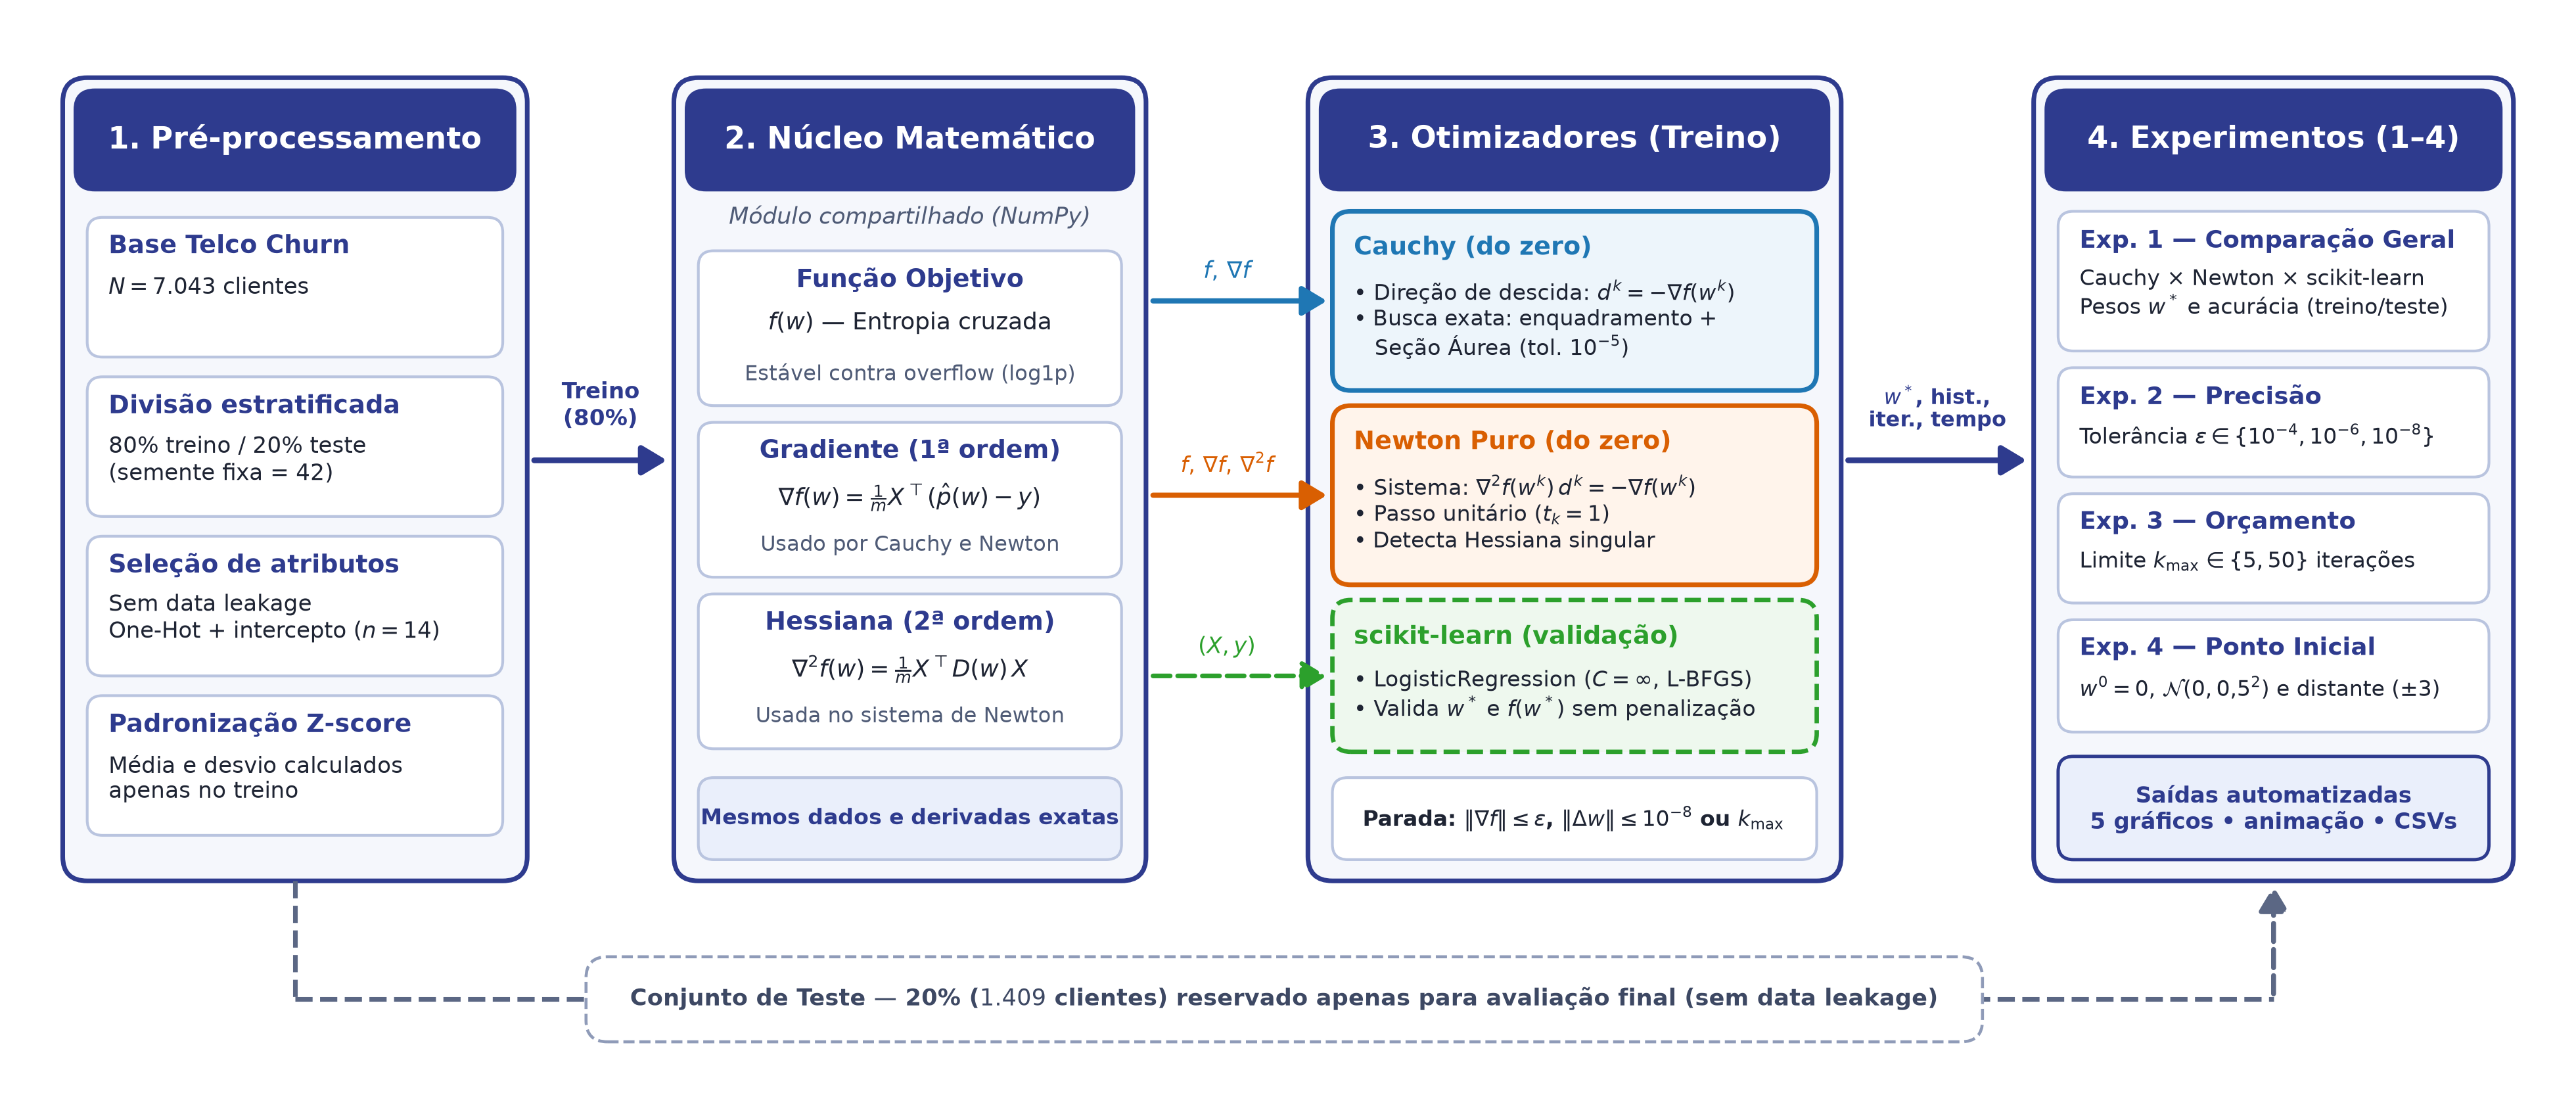
\includegraphics[width=\textwidth]{00_arquitetura_pipeline.png}
\caption{Arquitetura da implementação e fluxo experimental: pré-processamento sem vazamento de dados, núcleo matemático compartilhado, otimizadores e bateria de experimentos.}
\label{fig:arquitetura_pipeline}
\end{figure}

\FloatBarrier
\subsection{Experimento 1 --- Comparação geral dos métodos}

O primeiro experimento tem como objetivo comparar o desempenho dos métodos em uma configuração comum, partindo do vetor inicial $w^0 = 0$ e adotando tolerância de $10^{-6}$ para a norma do gradiente. Para a avaliação, foram considerados o valor final da função objetivo no conjunto de treino, a norma do gradiente, o número de iterações e o tempo de execução. Também foram calculadas as métricas de acurácia nos conjuntos de treino e teste. Os resultados obtidos são resumidos na Tabela~\ref{tab:exp1_comparacao}.

\begin{table}[htbp]
\centering
\caption{Comparação geral dos métodos no conjunto de treino ($w^0 = 0$ e tolerância $10^{-6}$).}
\label{tab:exp1_comparacao}
\renewcommand{\arraystretch}{1.15}
{\small
\begin{tabularx}{\textwidth}{@{} X r r r r @{}}
\toprule
\textbf{Método} & \textbf{Log-loss (treino)} & \textbf{Norma do gradiente} & \textbf{Iterações} & \textbf{Tempo} \\
\midrule
Cauchy & $0{,}367535$ & $9{,}60 \times 10^{-7}$ & $338$ & $1{,}634320$~s \\
Newton Puro & $0{,}367535$ & $1{,}32 \times 10^{-7}$ & $6$ & $0{,}004749$~s \\
\texttt{scikit-learn} & $0{,}367535$ & $1{,}54 \times 10^{-6}$ & $35$ & $0{,}022743$~s \\
\bottomrule
\end{tabularx}
}
\end{table}

Os três procedimentos obtiveram valores praticamente coincidentes para a função objetivo, aproximadamente 0,367535. Os coeficientes estimados também apresentaram concordância entre si, como ilustrado na Figura~\ref{fig:exp1_pesos}. Esse resultado indica que, nesta configuração, os métodos implementados encontraram soluções numéricas equivalentes à solução de referência do \texttt{scikit-learn}, dentro da precisão observada.

A principal diferença ocorreu no custo computacional, conforme ilustrado na Figura~\ref{fig:exp1_convergencia}. O método de Cauchy necessitou de 338 iterações e aproximadamente 1,63~s, enquanto Newton Puro atingiu o critério de parada em 6 iterações e aproximadamente 0,0047~s. A implementação do \texttt{scikit-learn} utilizou 35 iterações e aproximadamente 0,0227~s. Portanto, para esta base e este ponto inicial, Newton Puro apresentou a convergência mais rápida tanto em número de iterações quanto em tempo registrado. Essa vantagem deve ser interpretada no contexto desta dimensão do problema, pois cada iteração de Newton envolve o cálculo da Hessiana e a solução de um sistema linear.

No conjunto de teste, Cauchy e Newton Puro produziram \textit{log-loss} de aproximadamente 0,365378 e acurácia de 82,54\%. No conjunto de treino, a acurácia foi de aproximadamente 83,00\%. A proximidade entre os resultados de treino e teste sugere que não houve uma queda expressiva de desempenho na amostra reservada. A acurácia inicial, obtida antes do ajuste dos pesos, foi de aproximadamente 73,5\%, de modo que o modelo ajustado apresentou ganho de cerca de nove pontos percentuais.

\begin{figure}[htbp]
\centering
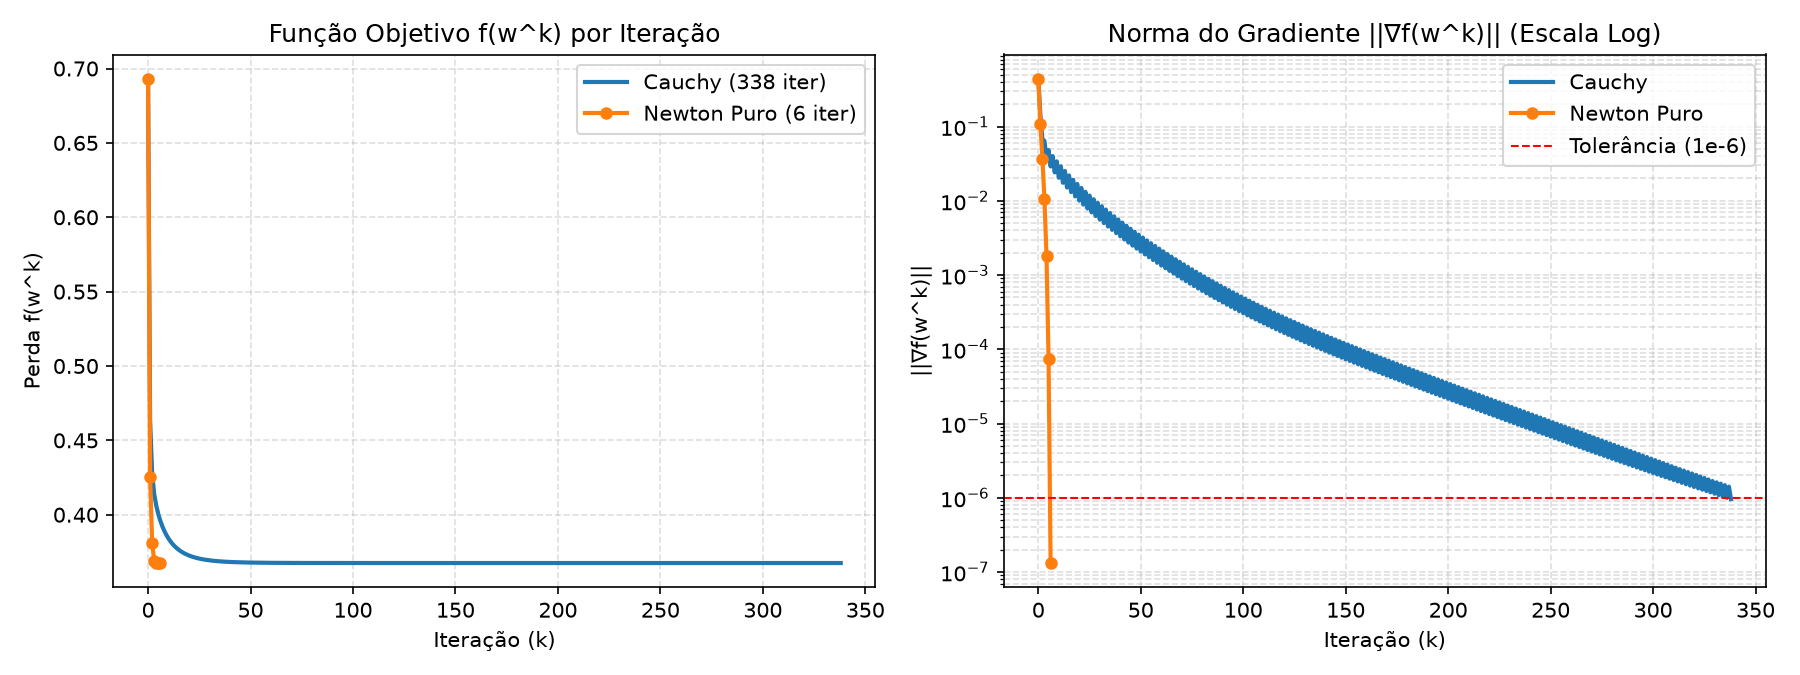
\includegraphics[width=\textwidth]{01_exp1_convergencia.png}
\caption{Evolução da função objetivo e da norma do gradiente ao longo das iterações para os métodos de Cauchy e Newton Puro.}
\label{fig:exp1_convergencia}
\end{figure}

\begin{figure}[htbp]
\centering
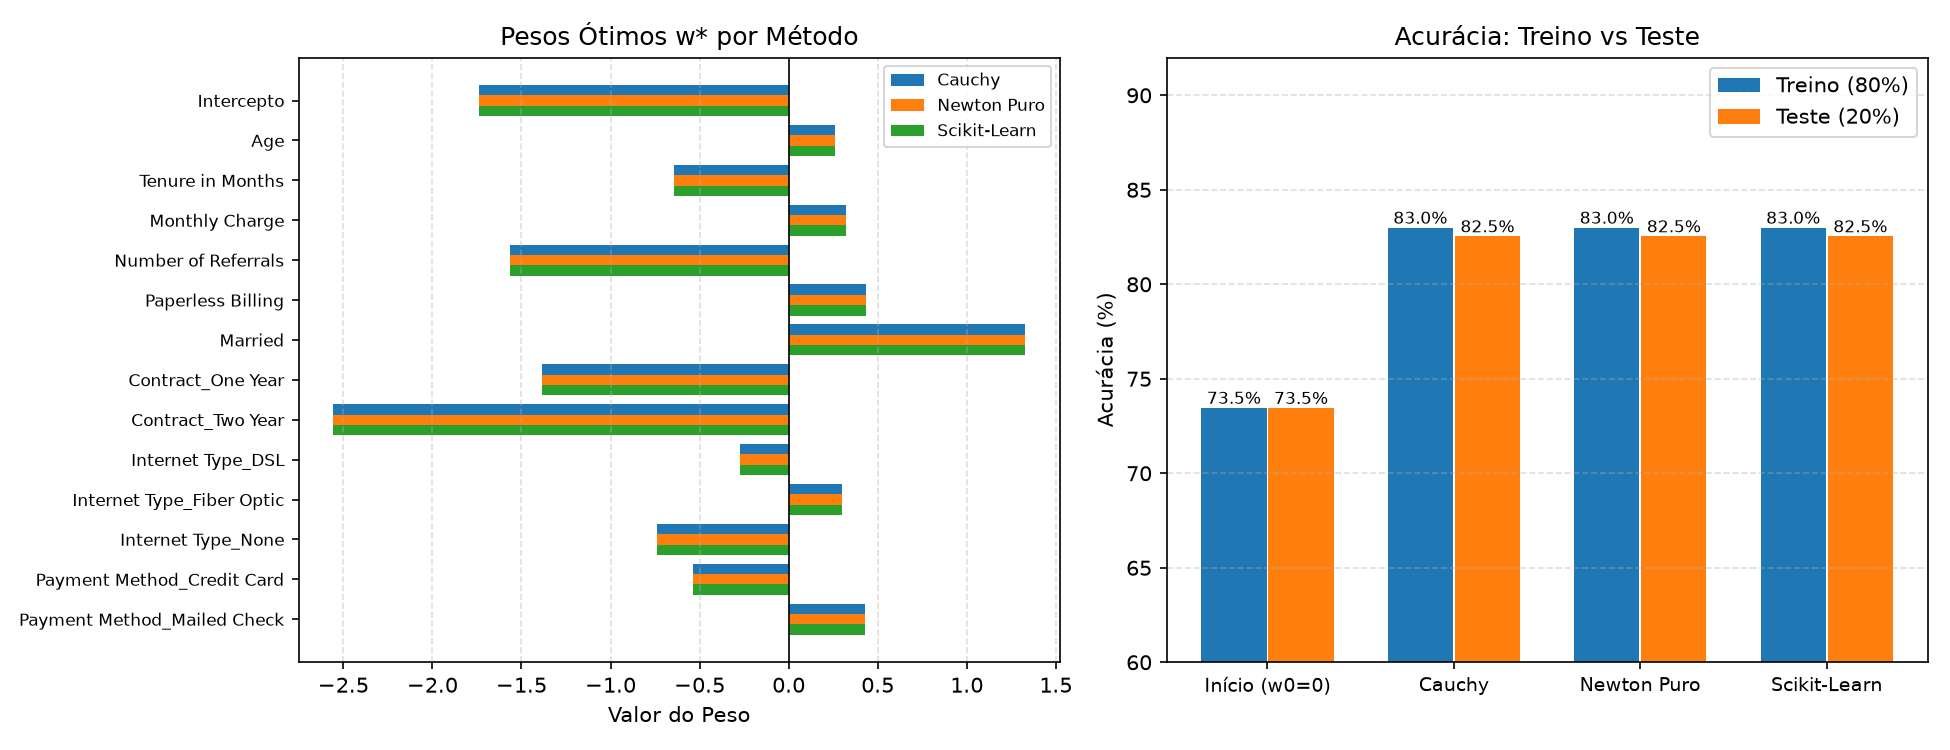
\includegraphics[width=\textwidth]{02_exp1_pesos_e_desempenho.png}
\caption{Comparação dos pesos estimados pelos três procedimentos e das acurácias nos conjuntos de treino e teste.}
\label{fig:exp1_pesos}
\end{figure}

Em conjunto, os resultados mostram que os dois métodos implementados alcançaram praticamente a mesma solução, mas com custos de convergência bastante distintos. O método de Newton Puro foi substancialmente mais eficiente nesta configuração, enquanto Cauchy apresentou uma trajetória mais longa e gradual. A concordância com o \texttt{scikit-learn} fornece uma verificação adicional da implementação da função objetivo e de suas derivadas.

\FloatBarrier
\subsection{Experimento 2 --- Influência da tolerância de convergência}

Neste experimento, investigou-se a influência da precisão exigida para a condição de parada. Foram utilizadas três tolerâncias para a norma do gradiente: $10^{-4}$, $10^{-6}$ e $10^{-8}$, mantendo-se o ponto inicial no vetor nulo e o limite máximo de iterações em 1.000. Assim, a única alteração entre as configurações foi o nível de precisão solicitado. Os resultados obtidos são apresentados na Tabela~\ref{tab:exp2_precisao}.

\begin{table}[htbp]
\centering
\caption{Desempenho dos métodos sob diferentes tolerâncias para a norma do gradiente ($w^0 = 0$ e máximo de 1.000 iterações).}
\label{tab:exp2_precisao}
\renewcommand{\arraystretch}{1.15}
{\small
\begin{tabularx}{\textwidth}{@{} l X r r r r @{}}
\toprule
\textbf{Configuração} & \textbf{Método} & \textbf{Iterações} & \begin{tabular}[b]{@{}r@{}}\textbf{Norma final}\\\textbf{do gradiente}\end{tabular} & \textbf{Log-loss} & \textbf{Tempo} \\
\midrule
2A / $10^{-4}$ & Cauchy & $140$ & $9{,}52 \times 10^{-5}$ & $0{,}367536$ & $0{,}7825$~s \\
2A / $10^{-4}$ & Newton Puro & $5$ & $7{,}50 \times 10^{-5}$ & $0{,}367535$ & $0{,}0042$~s \\
\addlinespace
2B / $10^{-6}$ & Cauchy & $338$ & $9{,}60 \times 10^{-7}$ & $0{,}367535$ & $1{,}7068$~s \\
2B / $10^{-6}$ & Newton Puro & $6$ & $1{,}32 \times 10^{-7}$ & $0{,}367535$ & $0{,}0046$~s \\
\addlinespace
2C / $10^{-8}$ & Cauchy & $580$ & $9{,}00 \times 10^{-9}$ & $0{,}367535$ & $2{,}8324$~s \\
2C / $10^{-8}$ & Newton Puro & $7$ & $4{,}24 \times 10^{-13}$ & $0{,}367535$ & $0{,}0051$~s \\
\bottomrule
\end{tabularx}
}
\end{table}

Observa-se que o aumento da exigência de precisão elevou o número de iterações dos dois métodos. Para Cauchy, o número de iterações passou de 140, com tolerância $10^{-4}$, para 338, com $10^{-6}$, e 580, com $10^{-8}$. Para Newton Puro, foram necessárias, respectivamente, 5, 6 e 7 iterações. Em todas as configurações, os métodos satisfizeram o critério de parada baseado na norma do gradiente.

Embora o valor final da função objetivo tenha permanecido praticamente constante, o custo computacional de Cauchy aumentou de aproximadamente 0,78~s para 2,83~s entre as tolerâncias extremas. Newton Puro manteve tempos próximos de 0,004 a 0,005~s. A Figura~\ref{fig:exp2_precisao} sintetiza o crescimento do número de iterações e do tempo de execução. Os resultados evidenciam que a exigência de maior precisão afeta de maneira mais intensa o método de Cauchy, enquanto Newton Puro manteve poucas iterações mesmo para a tolerância mais rigorosa.

\begin{figure}[htbp]
\centering
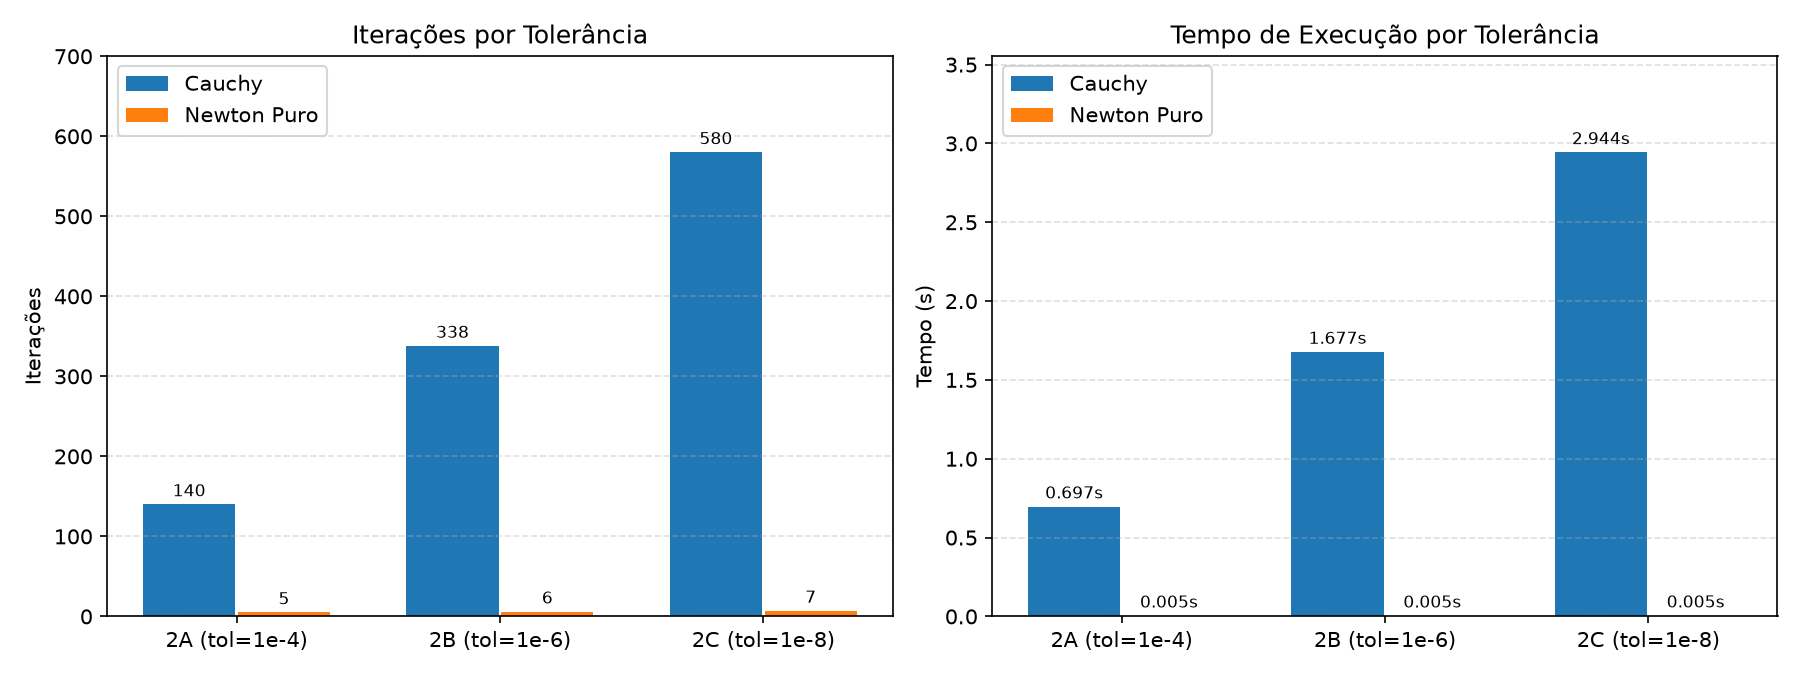
\includegraphics[width=\textwidth]{03_exp2_precisao.png}
\caption{Número de iterações e tempo de execução em função da tolerância da norma do gradiente.}
\label{fig:exp2_precisao}
\end{figure}

Portanto, para o problema considerado, Newton Puro mostrou menor sensibilidade ao aumento da precisão exigida em termos de quantidade de iterações e tempo de execução. Por outro lado, ambos os métodos convergiram para valores praticamente idênticos da função objetivo, indicando que a diferença observada está principalmente na eficiência do processo iterativo.

\FloatBarrier
\subsection{Experimento 3 --- Influência do limite máximo de iterações}

O terceiro experimento avaliou o comportamento dos métodos sob um orçamento limitado de iterações. Foram consideradas as configurações com máximo de 5 e 50 iterações, mantendo-se a tolerância do gradiente em $10^{-6}$ e o ponto inicial no vetor nulo. O objetivo foi verificar a proximidade da solução obtida quando o algoritmo dispõe de um número restrito de atualizações. Os resultados encontram-se na Tabela~\ref{tab:exp3_iteracoes}.

\begin{table}[htbp]
\centering
\caption{Desempenho dos métodos sob limites máximos de 5 e 50 iterações ($w^0 = 0$ e tolerância $10^{-6}$).}
\label{tab:exp3_iteracoes}
\renewcommand{\arraystretch}{1.15}
{\small
\begin{tabularx}{\textwidth}{@{} c X c r r r @{}}
\toprule
\begin{tabular}[b]{@{}c@{}}\textbf{Máximo}\\\textbf{permitido}\end{tabular} & \textbf{Método} & \textbf{Status} & \begin{tabular}[b]{@{}r@{}}\textbf{Iterações}\\\textbf{realizadas}\end{tabular} & \textbf{Log-loss} & \begin{tabular}[b]{@{}r@{}}\textbf{Norma final}\\\textbf{do gradiente}\end{tabular} \\
\midrule
$5$ & Cauchy & FALHOU & $5$ & $0{,}400423$ & $4{,}83 \times 10^{-2}$ \\
$5$ & Newton Puro & FALHOU & $5$ & $0{,}367535$ & $7{,}50 \times 10^{-5}$ \\
\addlinespace
$50$ & Cauchy & FALHOU & $50$ & $0{,}367840$ & $2{,}08 \times 10^{-3}$ \\
$50$ & Newton Puro & CONVERGIU & $6$ & $0{,}367535$ & $1{,}32 \times 10^{-7}$ \\
\bottomrule
\end{tabularx}
}
\end{table}

Com limite de 5 iterações, nenhum dos métodos atingiu a tolerância de $10^{-6}$. Ainda assim, Newton Puro alcançou \textit{log-loss} de aproximadamente 0,367535 e norma do gradiente de $7{,}50 \times 10^{-5}$, enquanto Cauchy apresentou \textit{log-loss} de 0,400423 e norma do gradiente de $4{,}83 \times 10^{-2}$. Portanto, mesmo sem satisfazer o critério de convergência, Newton Puro aproximou-se consideravelmente mais da solução nesse orçamento reduzido.

Quando o limite foi ampliado para 50 iterações, Newton Puro convergiu em 6 iterações, mantendo \textit{log-loss} de aproximadamente 0,367535. Cauchy utilizou as 50 iterações disponíveis, mas não atingiu a tolerância estabelecida, obtendo \textit{log-loss} de 0,367840 e norma do gradiente de $2{,}08 \times 10^{-3}$. A Figura~\ref{fig:exp3_iteracoes} apresenta a comparação da perda final e da norma do gradiente para os dois limites avaliados.

\begin{figure}[htbp]
\centering
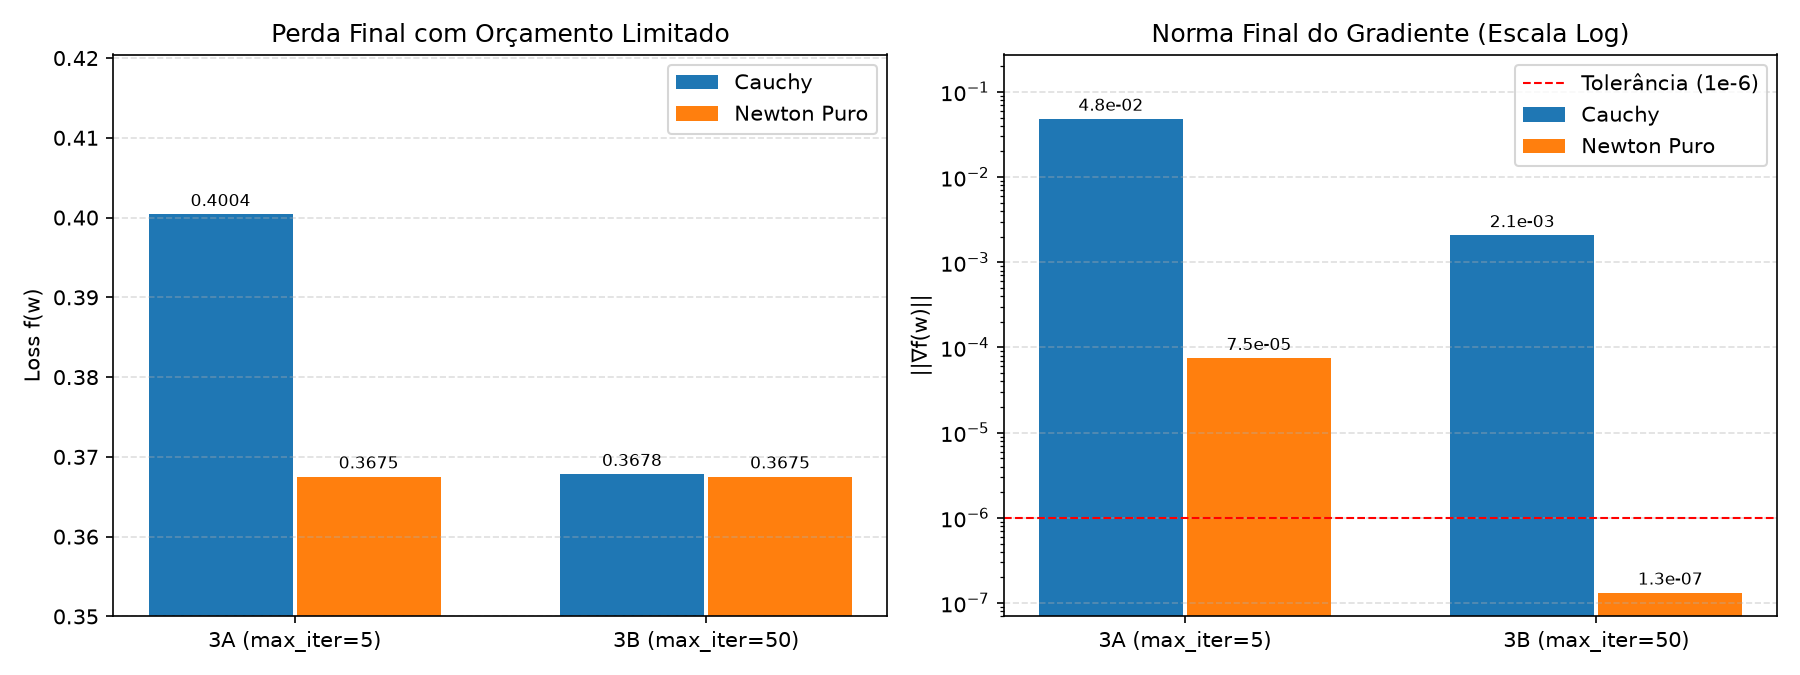
\includegraphics[width=\textwidth]{04_exp3_limite_iteracoes.png}
\caption{Log-loss final e norma do gradiente sob limites máximos de 5 e 50 iterações.}
\label{fig:exp3_iteracoes}
\end{figure}

Os resultados reforçam a diferença de velocidade de convergência observada nos experimentos anteriores. Newton Puro atingiu o critério de parada com poucas iterações, enquanto Cauchy necessitou de um número substancialmente maior de atualizações. Ressalta-se que o status de falha nas configurações em que o limite foi atingido indica apenas que o critério de parada não foi satisfeito dentro do orçamento definido, não significando necessariamente divergência do método.

\FloatBarrier
\subsection{Experimento 4 --- Sensibilidade ao ponto inicial}

Por fim, foi investigada a influência do ponto inicial sobre a convergência dos algoritmos. Foram testadas três condições: o vetor nulo, um vetor com componentes sorteadas segundo uma distribuição normal de média zero e desvio padrão 0,5, e um ponto inicial distante, com componentes de magnitude indicada no experimento por $\pm 3$. O objetivo foi avaliar se a escolha de $w^0$ altera o resultado final ou a estabilidade dos métodos. Os resultados estão resumidos na Tabela~\ref{tab:exp4_pontos_iniciais}.

\begin{table}[htbp]
\centering
\caption{Sensibilidade dos métodos à escolha do ponto inicial $w^0$ (tolerância $10^{-6}$).}
\label{tab:exp4_pontos_iniciais}
\renewcommand{\arraystretch}{1.15}
{\footnotesize
\setlength{\tabcolsep}{4pt}
\begin{tabularx}{\textwidth}{@{} X l c r r r r @{}}
\toprule
\textbf{Ponto inicial} & \textbf{Método} & \textbf{Status} & \textbf{Iterações} & \textbf{Log-loss} & \textbf{Norma final} & \textbf{Tempo} \\
\midrule
$w^0 = 0$ (origem) & Cauchy & CONVERGIU & $338$ & $0{,}367535$ & $9{,}60 \times 10^{-7}$ & $1{,}8223$~s \\
$w^0 = 0$ (origem) & Newton Puro & CONVERGIU & $6$ & $0{,}367535$ & $1{,}32 \times 10^{-7}$ & $0{,}0044$~s \\
\addlinespace
$w^0 \sim \mathcal{N}(0,\, 0{,}5^2)$ & Cauchy & CONVERGIU & $362$ & $0{,}367535$ & $9{,}81 \times 10^{-7}$ & $1{,}7630$~s \\
$w^0 \sim \mathcal{N}(0,\, 0{,}5^2)$ & Newton Puro & CONVERGIU & $6$ & $0{,}367535$ & $1{,}10 \times 10^{-8}$ & $0{,}0045$~s \\
\addlinespace
$w^0$ distante ($\pm 3$) & Cauchy & CONVERGIU & $426$ & $0{,}367535$ & $9{,}81 \times 10^{-7}$ & $2{,}0882$~s \\
$w^0$ distante ($\pm 3$) & Newton Puro & FALHOU & $2$ & $8{,}67 \times 10^{9}$ & $0{,}81$ & $0{,}0023$~s \\
\bottomrule
\end{tabularx}
}
\end{table}

Para os dois primeiros pontos iniciais, ambos os métodos convergiram para o mesmo valor de função objetivo, aproximadamente 0,367535. No caso do vetor nulo, Cauchy necessitou de 338 iterações, enquanto Newton Puro convergiu em 6. Para o ponto inicial aleatório, Cauchy utilizou 362 iterações e Newton Puro novamente convergiu em 6 iterações. Assim, pequenas perturbações em torno da origem não alteraram de maneira relevante a solução encontrada.

O comportamento foi diferente para o ponto inicial distante. Cauchy convergiu após 426 iterações, alcançando \textit{log-loss} de aproximadamente 0,367535. Newton Puro, por sua vez, interrompeu a execução após 2 iterações devido à singularidade numérica da Hessiana, com valor da função objetivo muito elevado. Esse resultado está de acordo com a limitação teórica discutida na Seção~\ref{subsubsec:newton}: o passo unitário do método puro não garante convergência global e, para pontos iniciais distantes, pode produzir iterandos em regiões numericamente desfavoráveis. A evolução da norma do gradiente nas três inicializações é ilustrada na Figura~\ref{fig:exp4_pontos_iniciais}.

\begin{figure}[htbp]
\centering
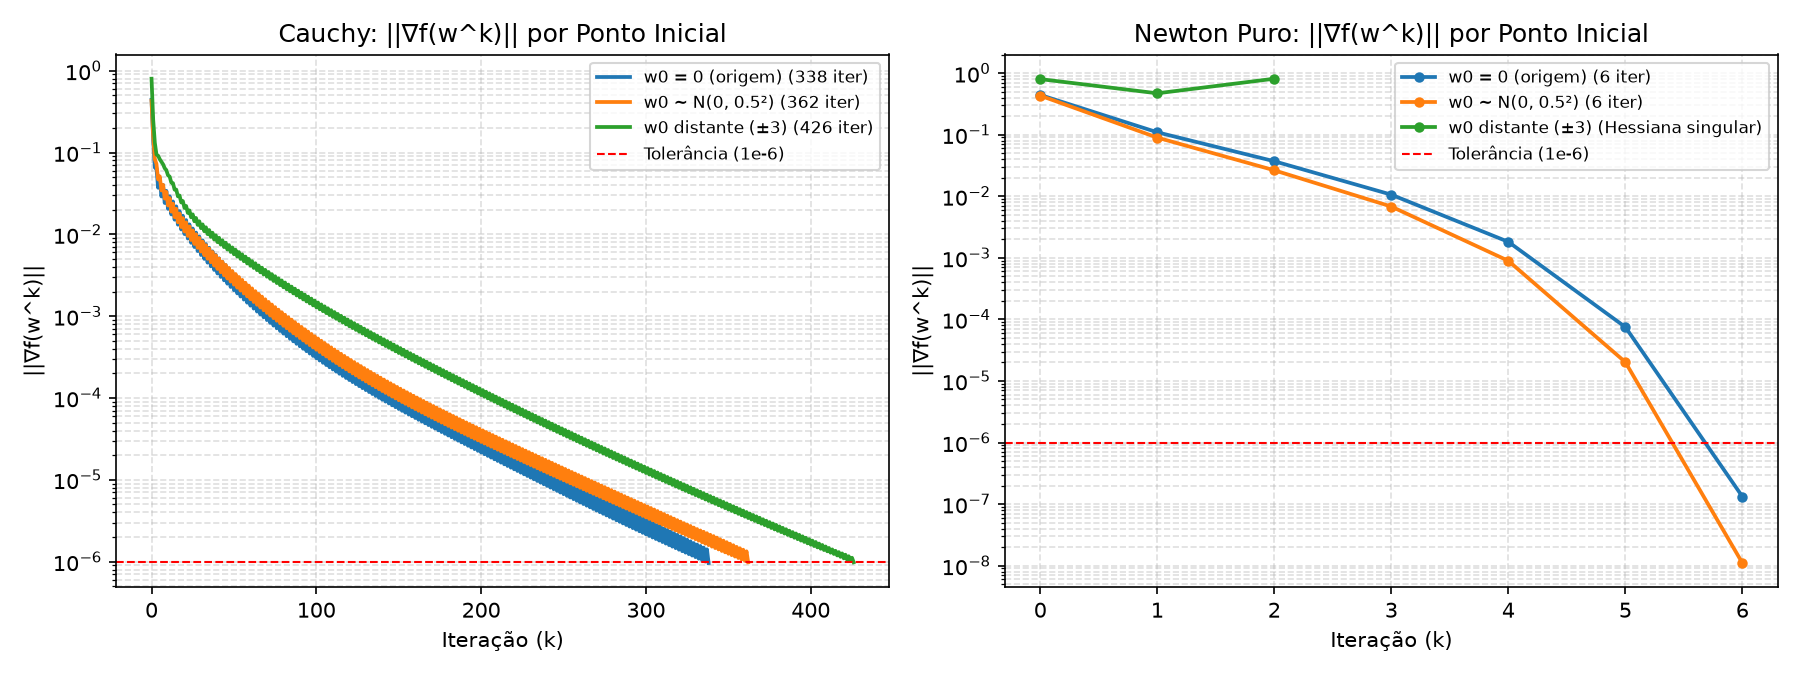
\includegraphics[width=\textwidth]{05_exp4_pontos_iniciais.png}
\caption{Evolução da norma do gradiente para diferentes pontos iniciais nos métodos de Cauchy e Newton Puro.}
\label{fig:exp4_pontos_iniciais}
\end{figure}

Dessa forma, o experimento evidencia uma diferença importante entre os métodos. Newton Puro apresentou convergência muito rápida quando iniciado em pontos próximos da solução, mas mostrou sensibilidade a uma inicialização distante. Cauchy apresentou convergência mais lenta, porém conseguiu alcançar a solução nas três condições testadas. Portanto, a eficiência de Newton Puro deve ser considerada em conjunto com sua menor robustez global na versão sem busca linear.

\FloatBarrier
\section{Conclusões}\label{sec:conclusoes}

Os experimentos numéricos corroboraram os resultados teóricos apresentados na Seção~\ref{subsec:metodos}. Nos cenários em que ambos convergiram, os métodos de Cauchy com busca linear exata via Seção Áurea e de Newton Puro produziram soluções equivalentes entre si e concordantes com a referência do \texttt{scikit-learn}, atingindo valores praticamente idênticos para a função objetivo e para os pesos estimados. Entretanto, o custo computacional para alcançar essa solução foi bastante distinto: Newton Puro exigiu poucas iterações e apresentou tempo de execução significativamente menor nas configurações em que convergiu, refletindo sua convergência quadrática local, enquanto Cauchy apresentou trajetória mais longa e gradual, característica da convergência linear.

A variação da tolerância confirmou que o aumento da exigência de precisão elevou o número de iterações dos dois métodos, porém de forma muito mais acentuada em Cauchy do que em Newton Puro. Sob orçamento limitado de iterações, Newton Puro também se aproximou muito mais rapidamente da solução ótima. Por outro lado, a análise de sensibilidade ao ponto inicial evidenciou na prática a principal limitação teórica do método de Newton Puro sem busca linear: a inicialização distante na região de saturação da sigmoide levou à singularidade numérica da Hessiana e à interrupção do algoritmo, ao passo que Cauchy, embora mais lento, convergiu em todas as inicializações avaliadas.

Em relação à capacidade preditiva, o modelo ajustado apresentou acurácia de aproximadamente 83,0\% no conjunto de treino e 82,5\% no conjunto de teste, com \textit{log-loss} de teste próxima de 0,3654, indicando comportamento consistente e boa generalização na divisão utilizada. Em síntese, os resultados mostram que Newton Puro é consideravelmente mais eficiente quando iniciado em uma região favorável, enquanto o método de Cauchy oferece maior robustez global diante de pontos iniciais distantes.

Como extensões naturais deste trabalho, seria interessante investigar versões globalizadas do método de Newton com busca linear inexata (como a condição de Armijo) ou estratégias de região de confiança, bem como métodos quase-Newton (como BFGS e L-BFGS) e a inclusão de regularização $L_2$ na função objetivo, de modo a combinar rapidez de convergência com robustez global e melhor condicionamento da Hessiana em problemas de maior dimensão.

\begin{thebibliography}{5}
\bibitem{ibm} IBM TEAM. \textit{Telco Customer Churn (11.1.3+)}. Proprietário: Al Fath Terry. 2024. Disponível em: \url{https://www.kaggle.com/dsv/8360350}. Acesso em: 1 nov. 2026.
\bibitem{ribeiro} RIBEIRO, A.; KARAS, E. \textit{Otimização Contínua: Aspectos Teóricos e Computacionais}. São Paulo: Cengage Learning, 2014.
\bibitem{agresti} AGRESTI, A. \textit{An Introduction to Categorical Data Analysis}. 3. ed. Hoboken: Wiley, 2018.
\bibitem{hastie} HASTIE, T.; TIBSHIRANI, R.; FRIEDMAN, J. \textit{The Elements of Statistical Learning: Data Mining, Inference, and Prediction}. 2. ed. New York: Springer, 2009.
\bibitem{pedregosa2011}
PEDREGOSA, F. et al. Scikit-learn: Machine Learning in Python. \textit{Journal of Machine Learning Research}, v.\ 12, p.\ 2825--2830, 2011.
\end{thebibliography}

\end{document}